In order to draw the feasible region, the following information is required:

\begin{align*}
	4x + y &\le 5 \\
	\therefore \text{Intersects axis at} (0,5) &\text{and} (1.25,0) \\
	5x - 2y &\le 3 \\
	\therefore \text{Intersects axis at} (0,-1.5) &\text{and} (0.6, 0) \\
	y &\le 3 \\
	\therefore \text{A line parallel to the x-axis at} y &= 3 \\
\end{align*}

It is also given that the feasible region occurs in the quadrant greater than
$x=-1$ and  $y=-1$.

\begin{figure}[H]
	\centering
	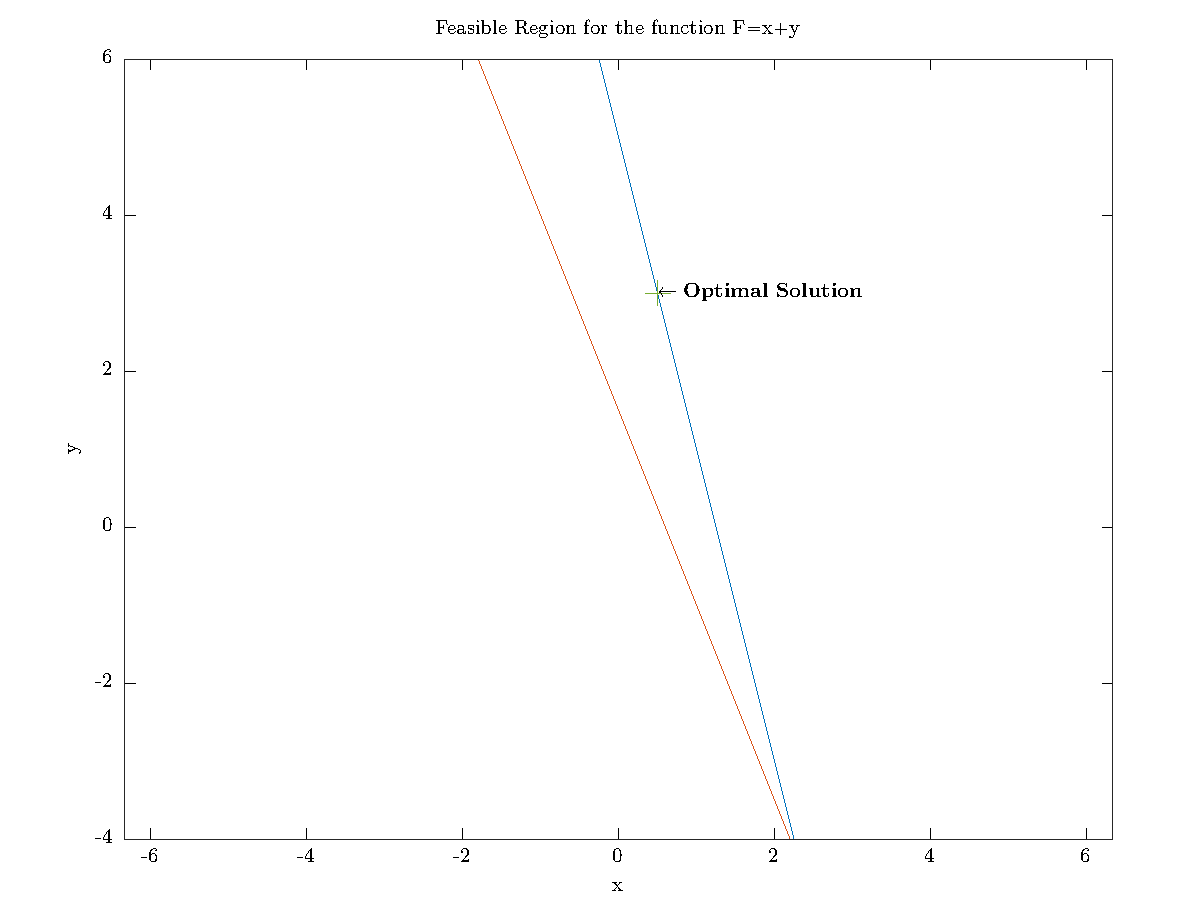
\includegraphics[width=\textwidth]{images/Q1}
	\caption{Feasible region for Q1}
	\label{fig:images-Q1}
\end{figure}

The maximum value is found to be at the point (0.5, 3.0).

If the objective function is changed to: minimise: $F=x$, the solution would be
(-1, 0), as the minimum value of x satisfies the objective function.
